\chapter{Modeling and Simulation}
\label{modeling}

This book is about modeling and simulating physical systems. Before we can build any models, it'll help to have a high-level understanding of what a model is. We'll also need to familiarize ourselves with the tools we use to build them. In this chapter, we'll look at the modeling process and introduce MATLAB, the programming language we'll use to represent models and run \mbox{simulations}. At the end of the chapter you'll find exercises you can use to test your knowledge.


\section{Modeling}

When I say ``modeling,'' I'm talking about something like Figure~\ref{fig:modeling}.
In the lower-left corner of the figure is the \emph{system}, something in the real world we're interested in.  Often, it's something complicated, so we have to decide which
details can be left out; removing details is called \emph{abstraction}.

\begin{figure}[h]
  \centerline{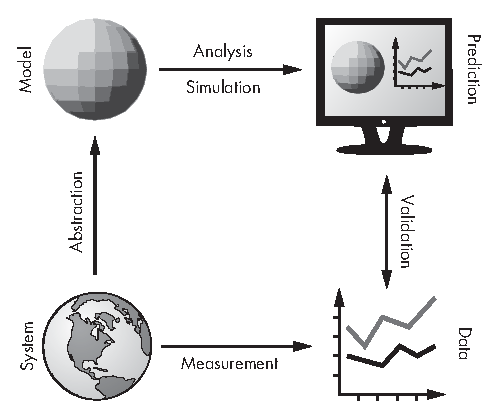
\includegraphics[scale=0.8]{images/figure01_01_new.eps}}
  \index{modeling}
  \caption{The modeling process}
  \label{fig:modeling}
\end{figure}

\index{system}
\index{abstraction}


The result of abstraction is a \emph{model}, shown in the upper left; a model is a description of the system that includes only the features we think are essential.  A model can be represented in the form of diagrams and equations, which can be used for mathematical analysis.  It can also be implemented in the form of a computer program, which can run simulations.

\index{model}
\index{simulation}
\index{analysis}

The result of analysis and simulation might be a prediction about what the system will do, an explanation of why it behaves the way it does, or a specific design engineered to satisfy a requirement or optimize performance.

\index{prediction}
\index{explanation}
\index{design}

We can validate predictions and test designs by taking measurements from the real world and comparing the data we get with the results from analysis and simulation.

\index{validation}
\index{data}

For any physical system there are many possible models, each one including and excluding different features or including different levels of detail.  The goal of the modeling process is to find the model best suited to its purpose (prediction, explanation, or design).

\index{iterative modeling}

Sometimes the best model is the most detailed.  If we include more features, the model is more realistic, and we expect its predictions to be more accurate. \index{realism}
But often a simpler model is better.  If we include only the essential features and leave out the rest, we get models that are easier to work with, and the explanations they provide can be clearer and more compelling. \index{simplicity}

As an example, suppose someone asked you why the orbit of the Earth is nearly elliptical.  If you model the Earth and Sun as point masses (ignoring their actual size), compute the gravitational force between them using Newton's law of universal gravitation, and compute the resulting orbit  using Newton's laws of motion, you can show that the result is an ellipse.\index{orbit}\index{ellipse}

Of course, the actual orbit of Earth is not a perfect ellipse, because of the gravitational forces of the Moon, Jupiter, and other objects in the solar system, and because Newton's laws of motion are only approximately true (they don't take into account relativistic effects).
\index{Newton}%
\index{relativity}%

But adding these features to the model would not improve the explanation; more detail would only be a distraction from the fundamental cause.  However, if the goal is to predict the position of the Earth with great precision, including more details might be necessary.

Choosing the best model depends on what the model is for.  It is usually a good idea to start with a simple model, even if it's likely to be too simple, and test whether it's good enough for its purpose.  Then you can add features gradually, starting with the ones you expect to be most essential.  This process is called \emph{iterative modeling}.

\index{iterative modeling}

Comparing the results of successive models provides a form of \emph{internal  validation} so you can catch conceptual, mathematical, and software errors.  And by adding and removing features, you can tell which ones have the biggest effect on the results, and which can be ignored.
\index{internal validation}%
\index{validation!internal}%
\index{external validation}%
\index{validation!external}%
Comparing results with data from the real world provides \emph{external validation}, which is generally the strongest test.

Figure~\ref{fig:modeling} shows that models can be used for both analysis and simulation; in this book we will do some analysis, but the focus is on simulation.  And the tool we will use to build simulations is MATLAB.  So let's get started.


\section{A Glorified Calculator}
\label{calc}

MATLAB is a programming language with features that support modeling and simulation.  It has a lot of features, so it can seem overwhelming, but at heart MATLAB is a glorified calculator.  When you start MATLAB you should see a window entitled MATLAB that contains smaller windows entitled Current Folder, Command Window, and Workspace.
In Octave, Current Folder is called File Browser.

\index{Command Window}
\index{workspace}
\index{interpreter}
\index{command}

\subsection{The Interpreter}
The Command Window runs the \emph{interpreter}, which allows you
to enter \emph{commands}; once entered, the interpreter executes the command and prints the
result.
Initially, the Command Window contains a welcome message with information
about the version of the software you're running, followed by a \emph{prompt}, which looks like this:\index{prompt}

\begin{code}
>>
\end{code}

The \lstinline{>>} symbol prompts you to enter a command.
The simplest kind of command is a mathematical \emph{expression},
like \lstinline{2 + 1}.\index{expression}
If you type an expression and then press \keycap{enter} (or \keycap{return}), MATLAB
\emph{evaluates} the expression and prints the result.

\begin{code}
>> 2 + 1
ans = 3
\end{code}

Just to be clear: in this example, MATLAB displayed \lstinline{>>}; I
typed \textbf{\lstinline{2 + 1}} and then hit \keycap{enter}, and MATLAB displayed \lstinline{ans = 3}.

\index{operator}
\index{operand}

In this expression, the plus sign is an \emph{operator} and the numbers \lstinline{2} and \lstinline{1} are \emph{operands}.
An expression can contain any number of operators and operands.  You
don't have to put spaces between them; some people do and some people
don't. Here's an example with no spaces:

\begin{code}
>> 1+2+3+4+5+6+7+8+9
ans = 45
\end{code}

Speaking of spaces, you might have noticed that MATLAB puts a blank
line between \lstinline{ans =} and the result.  In my examples I'll leave it out to  save room.

\index{multiplication}
\index{division}
\index{arithmetic operator}
\index{exponentiation}

The other arithmetic operators are pretty much what you would expect.
Subtraction is denoted by a minus sign (\lstinline{-}), multiplication is designated by
an asterisk (\lstinline{*}), division is denoted by a forward slash (\lstinline{/}).

\begin{code}
>> 2*3 - 4/5
ans = 5.2000
\end{code}

Another common operator is exponentiation, which uses the \lstinline{^}
symbol, sometimes called ``caret'' or ``hat.''  So, 2 raised to the
16th power is

\begin{code}
>> 2^16
ans = 65536
\end{code}

The order of operations is what you would expect from basic algebra:
exponentiation happens before multiplication and division, and multiplication and division happen before addition and subtraction.
If you want to override the order of operations, you can use parentheses.

\index{operations!order of}
\index{order of operations}
\index{parentheses}

\begin{code}
>> 2 * (3-4) / 5
ans = -0.4000
\end{code}

When I added the parentheses, I removed some spaces to make the
grouping of operands clearer to a human reader.  This is the first
of many style guidelines I will recommend for making your programs
easier to read.  Style doesn't change what the program does; the MATLAB
interpreter doesn't check for style.  But human readers do, and the
most important human who will read your code is you.

\index{debugging!First Theorem}

And that brings us to the First Theorem of Debugging:

\begin{quote}
Readable code is debuggable code.
\end{quote}

It's worth spending time to make your code pretty; it will save
you time \mbox{debugging}!


\subsection{Math Functions}

MATLAB knows how to compute pretty much every math function you've
heard of. For example, it knows all the trigonometric functions---here's how you
use them:

\index{math function!trigonometric}

\begin{code}
>> sin(1)
ans = 0.8415
\end{code}

This command is an example of a \emph{function call}.  The name of the
function is \lstinline{sin}, which is the usual abbreviation for the
trigonometric sine.  The value in parentheses is called the \emph{argument}.
\index{argument}%
\index{function!argument}%

The trig functions \lstinline{sin}, \lstinline{cos}, and  \lstinline{tan}---among many
others---work in radians, so the argument in the example is interpreted as 1~radian.
MATLAB also provides trig functions that work in degrees: \lstinline{sind}, \lstinline{cosd}, and \lstinline{tand}.

Some functions take more than one argument, in which case the arguments are
separated by commas.  For example, \lstinline{atan2} computes the inverse
tangent, which is the angle in radians between the positive x-axis and
the point with the given x- and y-coordinates.

\begin{code}
>> atan2(1,1)
ans = 0.7854
\end{code}

If that bit of trigonometry isn't familiar to you, don't worry about
it.  It's just an example of a function with multiple arguments.

\index{trigonometry}
\index{math function!exponential}

MATLAB also provides exponential functions, like \lstinline{exp}, which computes $e$ raised to the given power.  So \lstinline{exp(1)} is just $e$:

\begin{code}
>> exp(1)
ans = 2.7183
\end{code}

\index{math function!logarithm}

The inverse of \lstinline{exp} is \lstinline{log}, which computes the logarithm base $e$:

\begin{code}
>> log(exp(3))
ans = 3
\end{code}

This example also demonstrates that function calls can be \emph{nested};
that is, you can use the result from one function as an argument for
another.

\index{nested function call}
\index{function call!nested}
\index{operand}

More generally, you can use a function call as an operand in an \mbox{expression}.

\begin{code}
>> sqrt(sin(0.5)^2 + cos(0.5)^2)
ans = 1
\end{code}

As you probably guessed, \lstinline{sqrt} computes the square root.

\index{math function!square root}

There are lots of other math functions, but this isn't meant to
be a reference manual.  To learn about other functions, you should
read the documentation.


\section{Variables}

Of course, MATLAB is good for more than just evaluating expressions. One of the features that makes MATLAB more powerful than a calculator is the ability to give a name to a value.  A named value is called a \emph{variable}.

\index{variable}
\index{variable!predefined}
\index{predefined variable}

MATLAB comes with a few predefined variables. For
example, the name \lstinline{pi} refers to the
mathematical quantity $\pi$, which is approximately this:

\begin{code}
>> pi
ans = 3.1416
\end{code}

And if you do anything with complex numbers, you might find it
convenient that both \lstinline{i} and \lstinline{j} are predefined as the square
root of $-1$.

\index{complex number!imaginary unit}
\index{operand}
\index{expression}

You can use a variable name anywhere you can use a number---for example, as
an operand in an expression,

\begin{code}
>> pi * 3^2
ans = 28.2743
\end{code}
or as an argument to a function:

\begin{code}
>> sin(pi/2)
ans = 1
\end{code}

\index{argument}
\index{function call}

Whenever you evaluate an expression, MATLAB assigns the result to
a variable named \lstinline{ans}.  You can use \lstinline{ans} in a subsequent
calculation as shorthand for ``the value of the previous expression.''

\begin{code}
>> 3^2 + 4^2
ans = 25

>> sqrt(ans)
ans = 5
\end{code}

But keep in mind that the value of \lstinline{ans} changes every time
you evaluate an expression.


\subsection{Assignment Statements}

You can create your own variables, and give them values, with
an \emph{assignment statement}.  The assignment operator is the
equals sign (\lstinline{=}), used like so:

\index{assignment operator}
\index{operator!assignment}
\index{statement!assignment}

\begin{code}
>> x = 6 * 7
x = 42
\end{code}

This example creates a new variable named \lstinline{x} and assigns it the
value of the expression \lstinline{6 * 7}.  MATLAB responds with the
variable name and the computed value.

\index{expression}

There are a few rules when assigning variables a value. In every assignment statement, the left side has to be a legal variable name.  The right side can be any expression, including function calls.
\index{variable!name}%
\index{name!variable}%
\index{underscore}%
\index{case sensitive}%
Almost any sequence of lower- and uppercase letters is a legal
variable name.
Some punctuation is also legal, but the underscore (\lstinline{_}) is the only commonly used non-letter.
Numbers are fine, but not at the beginning.
Spaces are not allowed.  Variable names are
\emph{case sensitive}, so \lstinline{x} and \lstinline{X} are different variables.

Let's look at some examples of assignment statements.

\begin{code}
>> fibonacci0 = 1;

>> LENGTH = 10;

>> first_name = 'bob'
first_name = 'bob'
\end{code}

The first two examples demonstrate the use of the semicolon, which
suppresses the output from a command.  In this case MATLAB creates the
variables and assigns them values but displays nothing.
\index{syntax!semicolon}%
\index{semicolon}%
\index{suppress output}%
\index{output!suppress}%

The third example demonstrates that not everything
in MATLAB is a number.
A sequence of characters in single quotes is
a \emph{string}.

\index{string}
\index{character}

Although \lstinline{i}, \lstinline{j}, and \lstinline{pi} are predefined, you are free
to reassign them.  It's common to use \lstinline{i} and \lstinline{j} for other
purposes, but it's rare to assign a different value to
\lstinline{pi}.

\index{complex number!imaginary unit}


\subsection{Variables in the Workspace}

When you create a new variable, it appears in the Workspace window and is added to the \emph{workspace}, which is a
set of variables and their values.

\index{variable}
\index{workspace}

The \lstinline{who} command prints the
names of the variables in the workspace:

\index{who@\lstinline{who}}
% \index{command!\lstinline{who}}

\begin{code}
>> x = 5;
>> y = 7;
>> z = 9;
>> who

Your variables are:

x  y  z
\end{code}

The \lstinline{clear} command removes specified variables from the workspace:

\begin{code}
>> clear x
>> who

Your variables are:

y z
\end{code}

But be careful: if you don't specify any variables, \lstinline{clear} removes them all.

\index{clear@\lstinline{clear}}
\index{disp@\lstinline{disp}}

To display the value of a variable, you can use the \lstinline{disp} function:

\begin{code}
>> disp(z)
     9
\end{code}
but it's easier to just type the variable name:

\begin{code}
>> z
z = 9
\end{code}

Now that you've seen how to use them, let's take a step back and think about why we'd use variables.

\subsection{Why Variables?}

There are a number of reasons to use variables.\index{variable!reasons for}
A big one is to avoid recomputing a value you use repeatedly.  For
example, if your computation uses $e$ frequently, you might
want to compute it once and save the result.

\begin{code}
>> e = exp(1)
e = 2.7183
\end{code}

Variables also make the connection between the code and the underlying
mathematics more apparent.  If you're computing the area of a circle,
you might want to use a variable named \lstinline{r}:

\begin{code}
>> r = 3
r = 3

>> area = pi * r^2
area = 28.2743
\end{code}

That way, your code resembles the familiar formula $a = \pi r^2$.

You might also use a variable to break a long computation into a sequence of steps.
Suppose you're evaluating a big, hairy expression like this:

\begin{code}
p = ((x - theta) * sqrt(2 * pi) * sigma)^-1 * ...
exp(-1/2 * (log(x - theta) - zeta)^2 / sigma^2)
\end{code}

You can use an ellipsis to break the expression into multiple lines.
Just enter \lstinline{...} at the end of the first line and continue on to the
next.
\index{syntax!\lstinline{...}}
\index{ellipsis}But often it's better to break the computation into a sequence of
steps and assign intermediate results to variables:

\begin{code}
shiftx = x - theta
denom = shiftx * sqrt(2 * pi) * sigma
temp = (log(shiftx) - zeta) / sigma
exponent = -1/2 * temp^2
p = exp(exponent) / denom
\end{code}

The names of the intermediate variables explain their role in the
computation:  \lstinline{shiftx} is the value of \lstinline{x} shifted by
\lstinline{theta},  it should be no surprise that \lstinline{exponent} is the argument of \lstinline{exp}, and \lstinline{denom} ends up in the denominator.  Choosing informative names makes the code easier to read and understand, which makes it easier to debug.

\index{numerator}
\index{denominator}


\section{Errors}

\index{error}

Every error is a learning opportunity.
Whenever you learn a new feature, you should try to make as many errors as possible, as soon as possible.
When you make deliberate errors, you see what the error messages are.
Later, when you make accidental errors, you'll know what the messages mean.

Let's look at some common errors. A big one for beginners is leaving out the \lstinline{*}
for multiplication, as in this example:

\begin{code}
area = pi r^2
\end{code}

This code should produce the following error message:

\begin{stdout}
 area = pi r^2
           |
Error: Invalid expression. Check for missing multiplication
operator, missing or unbalanced delimiters, or other syntax
error. To construct matrices, use brackets instead of parentheses.
\end{stdout}
\index{invalid expression}%
\index{expression!invalid}%

The message indicates that the expression is invalid and suggests several things that might be wrong.
In this case, one of its guesses is right: we're missing a multiplication operator.

\index{parentheses}

Another common error is to leave out the parentheses around the
arguments of a function.  For example, in math notation it's common
to write something like $\sin \pi$, but in MATLAB if you write

\begin{code}
sin pi
\end{code}
you should get the following error message:

\begin{stdout}
Undefined function 'sin' for input arguments of type 'char'.
\end{stdout}

The problem is that when you leave out the parentheses, MATLAB treats
the argument as a string of characters (which have type \lstinline{'char'}).
In this case the error message is helpful, but in other cases the results can be baffling.
For example, if you call \lstinline{abs}, which computes absolute values, and forget the parentheses, you get a surprising result:

\begin{code}
>> abs pi
ans =  112   105
\end{code}

I won't explain this result; for now, I'll just suggest that you should \mbox{\emph{always}} put parentheses around arguments.

\index{error message}

Here's another common error.
If you were translating the mathematical expression
%
\[ \frac{1}{2 \sqrt \pi} \]
%
into MATLAB, you might be tempted to write this:

\begin{code}
1 / 2 * sqrt(pi)
\end{code}

But that would be wrong because of the order of operations.  Division and multiplication are evaluated from left to right, so this expression would multiply \lstinline{1/2} by \lstinline{sqrt(pi)}.

\index{order of operations}
\index{denominator}

To keep \lstinline{sqrt(pi)} in the denominator, you could use parentheses,

\begin{code}
1 / (2 * sqrt(pi))
\end{code}
or make the division explicit,

\begin{code}
1 / 2 / sqrt(pi)
\end{code}

\index{division}
\index{debugging!Second Theorem}

The last two examples bring us to the Second Theorem of Debugging:

\begin{quote}
The only thing worse than getting an error message is \emph{not} getting an error message.
\end{quote}

Beginning programmers often hate error messages and do everything they
can to make the messages go away.  Experienced programmers know that error
messages are your friend.  They can be hard to understand, and even
misleading, but it's worth the effort to understand them.

\section{Documentation}

MATLAB comes with two forms of documentation, \lstinline{help}
and \lstinline{doc}.
\index{documentation!doc@\lstinline{doc}}
\index{documentation!help@\lstinline{help}}The \lstinline{help} command works in the Command Window; just
enter \textbf{\lstinline{help}} followed by the name of a command.

% Here's an example where the output is in a stdout environment to
% avoid nonsensical syntax highlighting.

\begin{code}
>> help sin
\end{code}

You should see output like this:

\begin{stdout}
 sin    Sine of argument in radians.
    sin(X) is the sine of the elements of X.

    See also asin, sind, sinpi.
\end{stdout}

Some documentation uses vocabulary we haven't covered yet.
For example, \lstinline{the elements of X} might not make sense until
we get to vectors and matrices a few chapters from now.

\index{element}
\index{vector}
\index{matrix}

The \lstinline{doc} pages are usually better.
If you enter \lstinline{doc sin}, a browser window appears with more detailed information about the function, including examples of how to use it.  The examples often
use vectors and matrices, so they may not make sense yet,
but you can get a preview of what's coming.


\section{Chapter Review}

This chapter provided an overview of the modeling process, including abstraction, analysis and simulation, measurement, and validation.

It also introduced MATLAB, the programming language we'll use to write simulations.  So far, we've seen variables and values, arithmetic operations, and mathematical functions.

Here are a few terms from this chapter you might want to remember.

The \emph{interpreter} is the program that reads and executes MATLAB or \mbox{Octave} code.
It prints a \emph{prompt} to indicate that it's waiting for you to type a \emph{command}, which is a line of code executed by the interpreter.

An \emph{operator} is a symbol, like \lstinline{*} or \lstinline{+}, that
represents a mathematical operation.
An \emph{operand} is a number or variable that appears in an expression along
with operators.
An \emph{expression} is a sequence of operands and operators that specifies
a mathematical computation and yields a value.

A \emph{function} is a named computation; for example, \lstinline{log10} is the
name of a function that computes logarithms in base 10.
A \emph{function call} is a command that causes a function to execute and compute a result.
An \emph{argument} is an expression that appears in a function call to
specify the value the function operates on.

A \emph{variable} is a named value. An \emph{assignment statement} is a command that creates a new variable (if necessary) and gives it a value.
A \emph{workspace} is a set of variables and their values.

Finally, a \emph{string} is a value that consists of a sequence of characters (as opposed to a number).

In the next chapter, you'll start writing longer programs and learn about floating-point numbers.

\section{Exercises}

Before you go on, you might want to work on the following exercises.

\begin{ex}
\label{penny}
You might have heard that a penny dropped from the top of the Empire State Building would be going so fast when it hit the pavement that it would be embedded in the concrete or that if it hit a person it would break their skull.

\index{Empire State Building}
\index{penny}
\index{myth}

We can test this myth by making and analyzing a model.  To get started, we'll assume that the effect of air resistance is small.  This will turn out to be a bad assumption, but bear with me.

If air resistance is negligible, the primary force acting on the penny is gravity, which causes the penny to accelerate downward.

\index{air resistance}

If the initial velocity is 0, the velocity after $t$ seconds is $a t$, and the distance the penny has dropped is
%
\[ h = a t^2 / 2 \]
%
Using algebra, we can solve for $t$:
%
\[ t = \sqrt{ 2 h / a} \]
%
Plugging in the acceleration of gravity,
$a = \SI{9.8}{\meter\per\second\squared}$, and the height of the Empire State Building,
$h = \SI{381}{\meter}$, we get
$t = \SI{8.8}{\second}$.
Then, computing $v = a t$ we get a velocity on impact of $\SI{86}{\meter\per\second}$, which is about 190 miles per hour.  That sounds like it could hurt.

Use MATLAB to perform these computations, and check that you get the same result.
\end{ex}

\begin{ex}
The result in the previous exercise is not accurate because it ignores air resistance.  In reality, once the penny gets to about \SI{18}{\meter\per\second}, the upward force of air resistance equals the downward force of gravity, so the penny stops accelerating.  After that, it doesn't matter how far the penny falls; it hits the sidewalk at about \SI{18}{\meter\per\second}, much less than \SI{86}{\meter\per\second}.

As an exercise, compute the time it takes for the penny to reach the sidewalk if we assume that it accelerates with constant acceleration
$a = \SI{9.8}{\meter\per\second\squared}$ until it reaches terminal velocity, then falls with constant velocity until it hits the sidewalk.

The result you get is not exact, but it's a pretty good approximation.
\end{ex}
